\documentclass[11pt]{article}
% Course worksheet style copied verbatim from the inspected A1 source.
\usepackage[assignment]{style/worksheet}
\usepackage{longtable,booktabs,etoolbox,xurl}
% Unnumbered statements for Part 4's theory; numbers would collide with problem labels.
\usepackage{amsthm}
\theoremstyle{definition}
\newtheorem*{aTwoDefinition}{Definition}
\theoremstyle{plain}
\newtheorem*{aTwoLemma}{Lemma}
\newtheorem*{aTwoProposition}{Proposition}
\theoremstyle{remark}
\newtheorem*{aTwoRemark}{Remark}
\coursename{CS 312}
\setlength{\emergencystretch}{2em}
% This ungraded assignment has no point total. Keep the A1 title and typography.
\expandafter\patchcmd\csname\string\worksheettitle\endcsname
  {\totalpoints{} points}{}{}{
  \PackageError{a2}{Cannot patch worksheet title}{Check the shared title macro.}}
% The course name is the only byline field, so it needs no separator.
\makeatletter
\renewcommand{\ws@bylinesep}{}
\makeatother

% Parts 3 and 4 use subsection numbering; leave the shared A1 style intact.
\newcommand{\aTwoProblemNumber}{\arabic{question}}
\makeatletter
\patchcmd{\ws@problemlabel}{\arabic{question}}{\aTwoProblemNumber}{}{
  \PackageError{a2}{Cannot patch problem numbering}{Check the shared problem macro.}}
\makeatother

% Public course sweep-results project.
\newcommand{\providedSweepsURL}{https://wandb.ai/hashimoto-group/public-alchemy/overview}
\newcommand{\providedSweeps}{\href{\providedSweepsURL}{provided W\&B sweeps}}

\worksheetname{Assignment 2: Hyperparameter Scaling}

\begin{document}
\worksheettitle
\begin{shadebox}[Instructions.]
  This assignment is ungraded, but doing the assignment will significantly assist you in obtaining partial credit on your quiz. Submit a single PDF writeup to Gradescope by the deadline in the course schedule.

  \textbf{Please limit your PDF submission to 20 pages excluding the bonus question.}

For each problem, your deliverable will be two parts: an analysis of the provided experiments together with the new experiments requested in each problem, and a short (around one paragraph) synthesis of your interpretation of the experiments. Use both components to check and develop your understanding. Remember that \emph{you will be able to cite your assignment in your quiz to justify your answer} and so it is in your best interest to have a detailed and well-organized set of experiments that you fully understand in order to get partial credit on the quiz.

In the final, optional problem, you can develop an interesting outcome prediction problem akin to our quizzes, where you will submit a short code diff from our codebase (under 100 lines) and a prediction task, framed as either a single-answer or a multiple-answer multiple-choice question. If we choose to use your submitted quiz question in any way (including in some modified form) on the actual quiz, you will receive bonus points on the quiz equivalent to the value of the quiz question.
The example-question answer key is at the end of this handout.
\end{shadebox}

\unitheader{}{Overview}{}

Training neural networks requires us to reason about scale: we train larger models, use more data, and
increase batch sizes. Hyperparameters that work well at one scale may not work well
at another. In this assignment, you will study \emph{hyperparameter scaling}: how
to adjust hyperparameters as the model and training scale change.

This assignment addresses the following questions:
\begin{itemize}
\item How should hyperparameters like learning rate and weight decay scale as we train on more data?
\item Can initialization and learning-rate scaling let us reuse a single optimal learning rate as we scale?
\item How does scaling the batch size affect the hyperparameters?
\end{itemize}
The goal is to learn when experiments at one scale can guide training at another,
and how to test the limits of those scaling rules.

As part of this process, we will carefully study \emph{toy examples}: simple optimization tasks for which we have solid theory and predictions. Toy examples are important as they form the basis of many theory-based intuitions that researchers have, and understanding both the power and limitations of these models is critical to understanding the extent to which we should trust theory in deep learning optimization.

\begin{shadebox}[Our model.]
We use a Llama-style architecture with the following baseline dimensions:
8 layers, hidden size 512, 8 attention heads, a 4,096-token vocabulary, and about
35M parameters. The model uses query/key (QK) normalization, which applies root mean square
normalization to queries and keys within each attention head. The baseline context
length is 1,024 tokens. RoPE is unscaled and training uses a prefix
of the full source dataset shuffled with seed 42. We train on fresh data and
evaluate validation loss.
At the baseline model size and a batch size of 64 sequences, training on 614.4M
tokens takes approximately 15 minutes on a single H100.
\end{shadebox}

\subunitheader{Provided experiments}
Use the \href{\providedSweepsURL}{provided source sweeps} for Problems 1 and 2.
From the starter repository root, list the run links for a subpart with:
\begin{verbatim}
uv run python -m experiments.a2.provided_sweeps --part P1a --links
\end{verbatim}
Replace \texttt{P1a} with \texttt{P1b}, \texttt{P1d}, \texttt{P1e}, or \texttt{P2a} for the other supplied runs.
The command lists each run's token budget, optimizer, schedule, learning rate,
weight decay, and W\&B link.
Use the command without \texttt{-{}-links} to read the measurements offline.

\subunitheader{Estimated experiments}
The suggested grids total about 166 new runs, including 55 five-step tests;
supplied runs and optional explorations (including Muon) are excluded.
Reuse matching runs across parts. Stay within the \textbf{48 GPU-hour budget}:
plan for at most 36 hours of experiments and reserve 12 for debugging and reruns.
Time a representative run at each model size before launching sweeps; shrink
the grids as needed and report any untested comparisons.

\subunitheader{Default training settings}
Unless a problem specifies otherwise, use the following defaults for language-model
experiments. Write $\eta$ for the peak learning rate (LR) and $\lambda$ for the
weight-decay coefficient (WD). Each problem specifies its token budget.
The default model is $d8$, with the training settings below.

\begin{center}
\begin{tabular}{ll}
\toprule
Setting & Default \\
\midrule
Optimizer & AdamW \\
Peak learning rate $\eta$ & $.003$ \\
Weight decay $\lambda$ & $.1$ \\
Adam moment coefficients $(\beta_1,\beta_2)$ & $(.9,.95)$ \\
Numerical stabilizer $\epsilon$ & $10^{-8}$ \\
Batch size & 64 sequences \\
LR schedule & Linear decay after warmup \\
Warmup & First 1\% of training updates \\
Gradient clipping & Global gradient norm capped at 1 \\
Model and data seeds & 42 \\
\bottomrule
\end{tabular}
\end{center}

\subunitheader{AdamW: Adam with decoupled weight decay}
In this assignment, many of our problems will make use of AdamW. For completeness, we define what we mean by the AdamW optimizer here. AdamW combines an adaptive gradient update with a separate shrinkage of the weights.
At update $t\geq0$, let $g_t$ be the gradient supplied to Adam for a weight matrix $W_t$.
With moment coefficients $\beta_1,\beta_2$ and numerical stabilizer $\epsilon>0$,
define gradient and squared-gradient moments $m_t,v_t$, their bias-corrected
versions $\widehat m_t,\widehat v_t$, and the Adam direction $U_t$ below.
Start from $m_0=v_0=0$; operations are elementwise.
\[
\begin{aligned}
m_{t+1}&=\beta_1m_t+(1-\beta_1)g_t,
& v_{t+1}&=\beta_2v_t+(1-\beta_2)g_t^2,\\
\widehat m_{t+1}&=\frac{m_{t+1}}{1-\beta_1^{t+1}},
& \widehat v_{t+1}&=\frac{v_{t+1}}{1-\beta_2^{t+1}},\\
U_t&=\frac{\widehat m_{t+1}}{\sqrt{\widehat v_{t+1}}+\epsilon}.
\end{aligned}
\]
With current LR $\eta_t$,
AdamW updates the matrix as
\[
W_{t+1}=W_t-\eta_t U_t-\eta_t\lambda W_t.
\]
We follow the common practice of excluding embeddings, normalization parameters, and biases from weight decay.


\unitheader{A}{Learning-rate scaling with AdamW}{}

Optimal learning rates depend on other hyperparameters, such as batch size.
How should they change as we scale up the data or model?

We might imagine that there are many possible answers to this question. Since the model is the same, and the optimal learning rate is often fairly stable, we might imagine the optimal learning rate stays similar. Or, we might look at the theory of convex optimization and conclude that, based on the convergence theorems that the right thing to do would be to decrease learning rates at rates of $O(1/\sqrt{T})$ or $O(1/T)$ for $T$ steps.

This is a simple, but surprisingly complex and consequential topic. Even large scale, serious empirical efforts on this question leads to disagreement, as you can see in this example taken from the StepFun learning rate scaling paper.

\begin{center}
  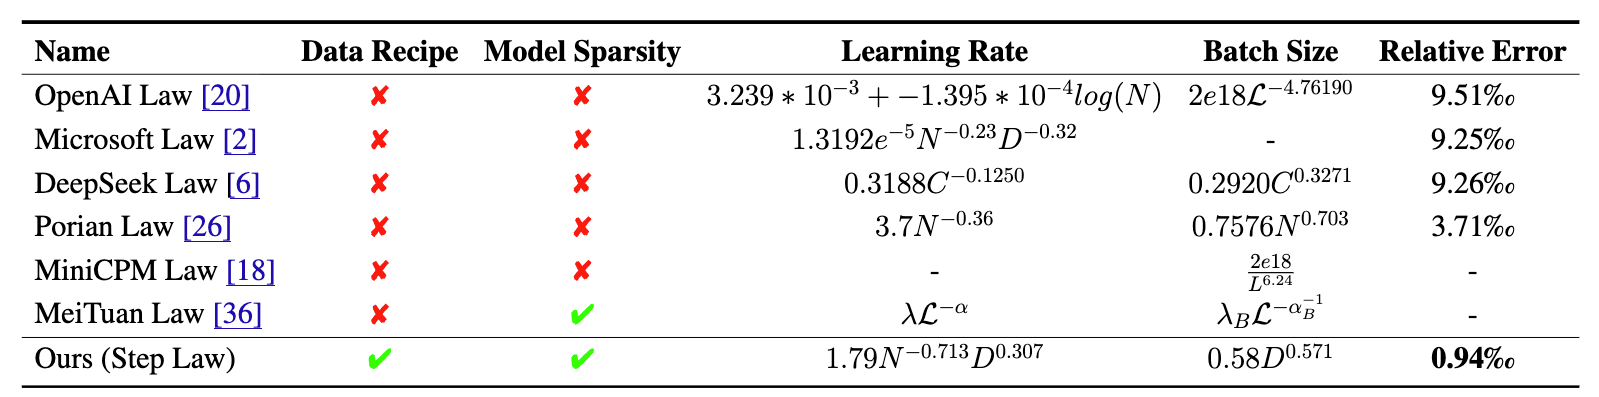
\includegraphics[width=0.78\linewidth]{figures/stepfun}\\
  {\footnotesize\itshape Examples of various \emph{scaling rules} for hyperparameters identified across the literature. Note the broad disagreement between credible papers and organizations.}
\end{center}

We will now study how learning rate scaling works in our $d8$ system and see if we can build intuition for what types of scaling rules are plausible. Throughout, let $D$ denote the training-token budget.

\needspace{16\baselineskip}
\begin{problem}{When can training on less data guide large scale runs? (9 new runs)}
Use the baseline model and default training settings above. Vary LR and the
training-token budget, keeping the other settings fixed.
For parts (a) and (b), analyze the \providedSweeps{} or the starter's CSV.
Fit the curves and make the plots yourself.

\begin{parts}
\item \textbf{Learn from small training budgets (provided runs).}
At 153.6M, 307.2M, and 614.4M tokens, investigate how final validation loss
changes with peak LR using the provided measurements at $\{.0015,.003,.006\}$. For each scale, fit a curve mapping peak LR to loss, and use this to estimate
the optimal LR. Use these optima to propose a scaling rule in the training-token budget.
Plot the fitted optima and your rule. What trend do you observe?

\needspace{4\baselineskip}
\item \textbf{Predict before increasing the budget (provided runs).}
Record your predicted optimal LRs at 1.2288B, 1.8432B, and 2.4576B tokens
before inspecting the provided measurements at these budgets.
Then fit their loss--LR curves and compare your predictions with the fitted optima. Does the trend from the small budgets continue?

\item \textbf{Compare and test two scaling rules (5 new runs).}
Fit one learning-rate power law over all six source budgets from parts (a) and (b),
and another over only 1.2288B, 1.8432B, and 2.4576B tokens.
Use each to predict the optimal LR at 4.9152B. Which prediction do you expect
to give the lower loss, and why?

Train at both predicted LRs and at target-grid LRs $\{.0015,.003,.006\}$.
Compare your predictions with the fitted target optimum and report their measured
loss gaps relative to the best sampled LR in the target grid. Did you find gains from using the smaller model fits? Think about bias-variance tradeoffs in fitting scaling laws, and how far you can extrapolate your scaling law fits.

\needspace{19\baselineskip}
\item \textbf{Hyperball versus AdamW (recommended: 4 new runs).}
The shape and predictability of learning rate scaling might vary significantly across optimizers, and one of the motivations for new and exotic optimization methods is that they may scale more predictably than the standard ones.

To this end we will explore Hyperball, which is a simple modification of the well-studied Adam optimizer. Hyperball uses an Adam direction but constrains each selected weight matrix to
keep its initial norm. For a linear-layer weight matrix $W_t$, let $U_{t}$ be Adam update direction. Write
$\lVert\cdot\rVert_F$ for the Frobenius norm (the square root of the sum of
squared entries). For nonzero norms, the Hyperball update is
\[
  W_{t+1}
=\frac{\lVert W_t\rVert_F}{\lVert\widetilde W_{t+1}\rVert_F}
\widetilde W_{t+1}
\qquad
\widetilde W_{t+1}
= W_t-\eta_t\frac{\lVert W_t\rVert_F}{\lVert U_t\rVert_F}U_t.
\]
We propose an update $\widetilde W_{{t+1}}$ by scaling the standard Adam update relative to the weight norm, and enforce that the norm remains the same after the step. Since hyperball already controls the norms, Hyperball uses no weight decay. Embeddings, normalization parameters, and biases use ordinary Adam.
The supplied runs use peak LR $(.000656/.00630)\eta\approx .1041\eta$ for
these Adam parameters, where $\eta$ is the listed Hyperball peak LR.
Apply the same warmup and decay multiplier to both groups, and keep this LR
ratio fixed in your target runs.

Use the 24 supplied Hyperball runs (\texttt{P1d}) at 153.6M, 307.2M,
and 614.4M tokens, with eight LRs at each budget. Fit an optimum at each
of these three budgets and fit a power law to those optima. Compare its trend
with AdamW fitted to the same three budgets; no larger Hyperball source budgets
are supplied. Record a prediction at 1.2288B tokens before running that target.
Test the predicted LR and three nearby LRs of your choice (up to four new runs,
reusing duplicates). Compare the prediction with the best sampled target loss.
Does the optimal LR vary more regularly with budget? Discuss the uncertainty
of extrapolating from only three source budgets.

\item \textbf{Explore schedule variants (optional).}
Thus far, we have studied optimal LR scaling for a single schedule. Do our findings transfer across learning rate schedules? Can we \emph{directly} transfer the optimal LR from one schedule to another?
Explore different learning-rate schedules, such as cosine decay or a constant
learning rate, using the same methodology.
\end{parts}
\end{problem}
\clearpage

\clearpage
\unitheader{B}{Joint learning-rate and weight-decay scaling}{}

At this point, you should have a general sense of how learning rates behave as a function of scale, and we've seen some intriguing signs in the hyperball experiment that learning rates and the \emph{norm} of the parameters might be related (at least in our transformer model). In this problem, we will dig deeper into the phenomenon and try to understand how learning rates and weight decay interact with each other.

\begin{problem}{How should learning rate and weight decay scale together? (4 new runs)}
\begin{parts}
\item \textbf{Let LR and WD vary together (provided runs).}
Analyze the \providedSweeps{} for the following LR--WD grids.
Our runs contain all combinations of peak LR and WDs given in the following table,
\begin{center}
\begin{tabular}{rll}
\toprule
Tokens (B) & Peak LRs & WDs \\
\midrule
.1536 & $\{.00075,.0015,.003\}$ & $\{.4,1.6,6.4\}$ \\
.3072 & $\{.0015,.003,.006\}$ & $\{.1,.4,.8\}$ \\
.6144 & $\{.0015,.003,.006\}$ & $\{.1,.2,.4\}$ \\
1.2288 & $\{.0015,.003,.006\}$ & $\{.1,.2,.4\}$ \\
\bottomrule
\end{tabular}
\end{center}

As we have two hyperparameters, we will have to extend our earlier scaling rules, and consider a bivariate functional form for the loss.
Let $x=\log\eta$ and $y=\log\lambda$. For each scale (token budget), fit a local quadratic $\widehat L(x,y)$ to approximate the final val loss using the coefficients
$a,b,c,d,e,f$:
\[
 \widehat L(x,y)=a+b x+c y+d x^2+e xy+f y^2,
\]
The cross term $e xy$ allows LR and WD to interact.

For each budget, draw its contours and mark the fitted optimum at each budget. If we make two plots, one for LR and WD where we plot optimal LR or WD as a function of scale, what do we see?
How does the LR trend compare with the one in Problem 1?
Can either coordinate be described well by a single power law?

Compare the best measured validation losses from joint tuning with those from Problem 1 at the same budgets. Plot both against tokens, along with their difference. How does the benefit of tuning WD depend on the training budget?

\item \textbf{From coupling to a joint scaling law (no new runs).}
At each budget, let $(\eta^*,\lambda^*)$ be the fitted optimal pair from part (a).
On its contour plot, draw your quadratic fit and observed data with the two axes being peak LR and WD (with log-log scale). Can increasing one hyperparameter compensate for decreasing another?
Draw a line where $\eta\lambda=\eta^*\lambda^*$ on this plot, and see how it relates to the contour plot.

Now plot $\eta^*\lambda^*$ against tokens and compare it with the separate
LR and WD trends. Does the product vary more regularly than either coordinate? Measure the $R^{2}$ of each of these different scaling fits and figure out which of these variables have the tightest power law scaling.

\needspace{4\baselineskip}
\item \textbf{Test the joint rule (4 new runs).}
Consider a policy with peak LR $.003$ at every budget (note that this is not asking for a constant LR schedule, we just fix the same peak LR across scales). Our goal will be to see if we can ``rescue'' this LR policy by adjusting our weight decay.

\begin{enumerate}[label=\arabic*., nosep, leftmargin=*]
\item \textbf{Fit.} Use the product law from part (b) fitted on
$\{.1536,.3072,.6144,1.2288\}$B tokens.
\item \textbf{Test.} Validate at \textbf{2.4576B tokens}, excluded from the fit.
At peak LR $.003$, test the WD given by the predicted product divided by $.003$.
Use linear decay for all runs.
\item \textbf{Compare.} Use two baselines, both trained for 2.4576B tokens:
(i) reuse the LR--WD pair with the lowest validation loss in the 153.6M sweep,
without retuning; (ii) fix peak LR at $.003$, test WD $\{.05,.1,.2\}$,
and take the best validation loss.
Report the prediction's loss gap to both baselines.
Does the product rule give an effective training recipe?
\end{enumerate}
\end{parts}
\end{problem}
\clearpage
\begin{examplequestion}[difficulty=medium]
\phantomsection\label{ex:a2-wd-timing}
\textbf{Can we postpone weight decay?}
Use the default training settings at 153.6M tokens with peak LR $.0015$ and WD $\lambda=.4$, with initialization seeds 42--44 and fixed data order. We modify the standard training process so that weight decay does not happen at every step, but instead applies a stronger weight decay every $K$ steps.

Let $\eta_t$ be the LR actually used at update $t$ (the optimizer's LR
before calling \texttt{optimizer.step}, not the LR after advancing its scheduler).
With positive warmup the first update uses zero LR, and the schedule reaches
zero only after the final update. Ordinary AdamW scales down the weights by $r_t=1-\eta_t\lambda$ before applying
the gradient update. Compare three schedules:
\begin{itemize}
\item Apply weight decay every update, as usual.
\item Apply it only at the end of each block of two updates.
\item Apply it only at the end of each block of four updates.
\end{itemize}
For a block ending at update $t$ with length $k$, the delayed schedule applies a stronger weight decay every $k$ steps
\[
 \widetilde r_t=\prod_{j=t-k+1}^{t}(1-\eta_j\lambda).
\]

The usual schedule gives mean final validation loss approximately $3.209$
across the three seeds.
\textbf{Predict the mean final validation loss for each delayed schedule.}
Round each mean to the nearest multiple of $0.01$.
\begin{itemize}
\item Weight decay every two updates: \underline{\hspace{2cm}}.
\item Weight decay every four updates: \underline{\hspace{2cm}}.
\end{itemize}
\end{examplequestion}


\clearpage
\unitheader{C}{How does batch size affect the hyperparameters?}{}

We now have had some taste of bivariate hyperparameters scaling (in our learning rate and weight decay tuning problem). We might wonder whether if there is a better way, where we can mathematically derive the right scaling relationships between hyperparameters.

To this end, we will study how batch size, learning rate, and scale all interact with each other. Batch size is an ideal variable to study, since the relationship between batch size, learning rates and convergence rates are very well studied and understood as part of the theory of online optimization.

We will make use of a well-known toy model called the noisy quadratic model, and see how this gives us learning-rate rules that (might) carry over to language model training in the wild.

\begingroup
\setcounter{question}{0}
\renewcommand{\aTwoProblemNumber}{3.\arabic{question}}

\subunitheader{Background: The noisy quadratic model}

A noisy quadratic model (NQM) replaces neural-network training with a quadratic
loss and noisy gradients. There are two key properties of the noisy quadratic that we will need to vary and understand. The curvature of the quadratic controls the optimization difficulty of the problem, and controls how quickly different directions
can be optimized; the gradient noise represents variation among training examples and informs whether larger batches are helpful.
We will follow
\href{https://proceedings.neurips.cc/paper_files/paper/2019/hash/e0eacd983971634327ae1819ea8b6214-Abstract.html}{Guodong Zhang et al. (2019),
\emph{Which Algorithmic Choices Matter at Which Batch Sizes? Insights From a
Noisy Quadratic Model}}, which uses this simple model to explain how learning
rate, momentum, and the optimizer affect batch-size scaling.

We will investigate two conclusions and the conditions under which they hold:
\begin{enumerate}[label=\arabic*.]
\item \textbf{Optimal LR can follow a power law in batch size.}
Let $B$ be batch size and $\eta^*(B)$ the LR minimizing expected final loss
at a fixed total number of training examples. Write a candidate rule as
$\eta^*(B)\approx cB^p$, with fitted constants $c$ and $p$.
For SGD in the small-step regime, the NQM predicts approximately linear scaling,
        $p=1$: doubling batch size calls for doubling LR. Of course, there will come a point where this prediction breaks down, as an arbitrarily large learning rate will lead to divergence. We will test this scaling rule, and identify the range of parameters where it is useful.
\item \textbf{Momentum can help more at large batches than at small batches.}
The classical NQM prediction is that, in the noise-dominated small-batch regime,
SGD momentum mainly rescales the effective LR and offers little extra benefit
after LR tuning. At larger batches, reduced noise can allow momentum to
accelerate convergence. We will test this prediction at a finite training budget and perform comparisons with Adam.
\end{enumerate}


Our first problem will make use of a simple, two dimensional quadratic model for you to play with.
\paragraph{2D quadratic toy model.}
Let $w=(w_1,w_2)^\top$ be the parameters and fix the curvature matrix
$H=\operatorname{diag}(1,10)$. The loss and its exact gradient are
\[
 f(w)=\tfrac12 w^\top H w=\tfrac12(w_1^2+10w_2^2),
 \qquad \nabla f(w)=Hw.
\]
To define the \emph{noisy} part of this quadratic, we will consider our gradients to be noisy version of the true gradient. For an update with batch size $B$, we define the corresponding minibatch gradient to be
\[
 g_t=Hw_t+\epsilon_t,\qquad
 \epsilon_t\sim\mathcal N(0,I_2/B)
\]
independently across updates, where $I_2$ is the two-dimensional identity matrix. This noise model comes from the naive assumption that the gradients are averages of i.i.d. items, and thus we expect variance to scale as $O(1/B)$.

\paragraph{Optimizers.}
In this problem, we will use a simplified optimizer model with constant LR $\eta$ and no weight decay. For the optimizer itself, we will study Stochastic gradient descent (SGD)  (defined as $w_{t+1}=w_t-\eta g_t$), Adam with $\epsilon=10^{-8}$, $\beta_{1}=0.9$, and $\beta_{2}=0.95$, and RMSProp, which is Adam with $\beta_{1}=0$.

\begin{problem}{What does this model predict about batch size? (Run locally with CPUs)}
  Consider our 2D toy quadratic model above. You will perform stochastic optimization on this toy model using the noisy gradients and compare how the hyperparameters change the final loss.

    Concretely, let $N=8,192$ be the total dataset size, $B$ be the batch size (which we specify below), and  $w_{0,1}\sim\mathcal N(0,1)$ and $w_{0,2}\sim\mathcal N(0,.1)$ as initialization.

     Compare expected final loss $L_N(B,\eta)=\mathbb E[f(w_{N/B})]$, estimated by averaging over independent
     initializations and noise (using at least 512 samples).

  \begin{parts}


\item \textbf{SGD.}
Sweep LR at batches $B\in\{1,2,4,8,16,32,64\}$ and fit a power law to the
estimated optimal LRs. Predict the optimal LR at $B=256$, then test the
prediction with an LR sweep at that batch. Extend the batch range through
512 and plot optimal LR and best final loss after tuning LR.
Over what range does the rule work? Think about how reduced gradient noise
competes with fewer updates at fixed $N$.

\item \textbf{Adaptive updates.}
Repeat the experiment with RMSProp and Adam, tuning LR separately.
Compare the source exponents and the losses at predicted versus tuned LRs
at batch 256. Do these optimizers follow the same rule, and does a similar exponent imply similar transfer accuracy?
State your predictions for the language model setting. How should optimal LR change with batch size, and over what range do you expect that prediction to hold?

\item \textbf{Explore the assumptions.}
Replace the gradient-noise covariance $I_2$ by $\sigma^2 I_2$ for
$\sigma\in\{1,\allowbreak 10,\allowbreak 100,\allowbreak 300\}$. Repeat the RMSProp and Adam source fits and
batch-256 tests. Plot the fitted exponent against $\sigma$.
Does changing the ratio of gradient signal to noise change the scaling rule?
Relate your observations to the contributions to the second moment.

As a curvature comparison, repeat the experiments with the scalar loss $f(w)=w^2/2$, initial $w_0\sim\mathcal N(0,2)$, and gradient-noise variance $\sigma^2/B$. Which conclusions
are sensitive to the curvature model?

\item \textbf{Momentum at small and large batches.}
Return to $H=\operatorname{diag}(1,10)$ and noise covariance $I_2$.
For SGD with momentum, initialize $s_0=0$ and use
\[
 s_{t+1}=\mu s_t+g_t,\qquad w_{t+1}=w_t-\eta s_{t+1},
\]
where $\mu$ is the momentum coefficient.
At small batch $B=16$ and large batch $B=256$, compare $\mu=0$ and $.9$,
tuning LR separately. For Adam, keep $\beta_2=.95$ and jointly sweep
$\beta_1$ and LR at each batch (hint: you should include $\beta_{1}=0$, $0.9$ and other values closer to one).

Plot the best loss at each $\beta_1$ after tuning LR.
How does the benefit of momentum depend on batch size? Compare the learning
curves of the best ($\beta$, LR) pair with the best no-momentum baseline. Do you expect these observations to carry over to language model training?

\end{parts}
\end{problem}

\clearpage
\subunitheader{Batch size scaling in a language model}

Do the scaling rules and momentum effects from the NQM carry over to
language-model training? Use the default model and training settings at
614.4M tokens, varying batch size and the specified hyperparameters.

Here $B$ is the number of sequences per optimizer update. Use microbatches of
$\min(B,64)$ sequences and report the actual number of tokens processed.
Use a linear learning-rate schedule with warmup over the first 1\% of
optimizer updates. The batch-switch example below specifies its own
schedule in terms of tokens processed.


\begin{problem}{What should scale when batch size changes? (suggested: 48 new runs)}
\begin{parts}
\item \textbf{Tune LR with weight decay (9 new runs).}
Set WD to $.1$ and sweep peak LR at $B\in\{8,16,32,64\}$.
Plot the loss--LR curves, fitted optimal LR, and best measured loss against
batch size. How do the optimal LR and performance change with batch size?

\item \textbf{Compare two scaling hypotheses (suggested: 27 new runs).}
The NQM can also give predictions of how weight decay and batch might jointly scale together.
Design experiments at $B\in\{8,16,32,64\}$ to test two hypotheses:
\begin{enumerate}[label=\roman*.]
\item Fix WD at $.1$ across batches and scale the optimal peak LR.
\item Fix peak LR at $.0015$ across batches and scale the optimal WD.
\end{enumerate}
Use the source results to predict configurations at $B=128$ and $B=256$,
then test which hypothesis transfers better. Discuss whether your findings
agree with the NQM.

\item \textbf{Ablate momentum (suggested: 12 new runs).}
At $B=8$ and $B=256$, hold each batch's best measured LR--WD pair and
$\beta_2=.95$ fixed. Design experiments including a $\beta_1=0$ control to test how the effect of momentum changes with batch size.
Compare with our earlier problem when we retuned LR.

\item \textbf{What does the NQM explain? (no new runs).}
Which predictions from your quadratic experiments agree with your language-model experiments,
and which do not?

Give a short prediction--measurement table for LR--batch-size scaling,
weight decay, and momentum. Include the measured target losses supporting
your conclusions. Distinguish a prediction that fails from an effect
the NQM does not model. What would you change in the NQM to explain one of
the disagreements?
\end{parts}
\end{problem}

\paragraph{Further reading.}
\href{https://arxiv.org/abs/2505.13738}{\textbf{Power Lines}}: WD--LR--batch coupling;
\href{https://arxiv.org/abs/2503.04715}{\textbf{Step Law}}: optimal LR and batch-size scaling;
\href{https://arxiv.org/abs/2606.16899}{\textbf{Hyperball}}: control of weight and update norms.

\endgroup
\setcounter{question}{3}

\clearpage
\begin{examplequestion}[difficulty=hard]
\phantomsection\label{ex:a2-batch-switch}
\textbf{Double batchsize during training}
Train the $d8$ language model 614.4M tokens with AdamW,
initial batch size $64$, peak LR $.0015$, and WD $1.6$.
Let $\eta_{\rm base}(D)$ denote the learning rate after processing
$D$ tokens: warm up over the first $1\%$ of tokens, then decay linearly to zero
at 614.4M tokens.

After processing exactly 307.2M tokens, double the batch size to $128$.
Reach the midpoint with 4,687 batches of 64 sequences followed by one batch
of 32; this gives 4,688 updates before the switch. Then use 2,343 batches of
128 sequences and a final batch of 96, giving 2,344 updates after the switch.
Compute each update's mean loss using its actual batch size.
Keep Adam's accumulated moments and both $\beta$ values unchanged.
For the remaining half of training, consider five policies:
\begin{center}
\begin{tabular}{clcc}
\toprule
Policy & Change at the midpoint & LR after the change & WD after the change\\
\midrule
A & Neither LR nor WD & $\eta_{\rm base}(D)$ & $1.6$\\
B & Multiply LR by $\sqrt{2}$ & $\sqrt{2}\,\eta_{\rm base}(D)$ & $1.6$\\
C & Multiply LR by $2$ & $2\,\eta_{\rm base}(D)$ & $1.6$\\
D & Multiply WD by $\sqrt{2}$ & $\eta_{\rm base}(D)$ & $1.6\sqrt{2}$\\
E & Multiply WD by $2$ & $\eta_{\rm base}(D)$ & $3.2$\\
\bottomrule
\end{tabular}
\end{center}
All runs process the same ordered tokens. Evaluate $\eta_{\rm base}(D)$ at
the number of tokens consumed \emph{before} each update, including the partial
batches. Changing the batch size must not restart warmup.
\textbf{Which policy do you predict will give the lowest mean final validation loss across 3 seeds (42,43,44)?}
Choose one and explain how changing LR or WD affects training when there are approximately half as many optimizer updates per token after the switch.
\end{examplequestion}



\clearpage
\unitheader{D}{Part 4: Initialization, feature learning, and transfer}{}

So far, we have relied on a scaling-law based approach to finding good hyperparameters at large scale. However, even a theory-guided approach of this kind may seem unsatisfying. Why does the optimal hyperparameter have to change at all? If we design the architecture and optimizer right, perhaps we could tune a hyperparameter once, and use that same optimal hyperparameter everywhere. This is the promise of various hyperparameter transfer schemes, and we will go in-depth into a popular kind of transfer scheme known as $\mu P$.

\subunitheader{The goal and the $abc$ parameterization}
We want to tune hyperparameters on a small model and reuse them as we scale width
and depth. It will turn out that we can patch up existing architectures and optimizers to have reasonable hyperparameter transfer by adjusting some small details in how we parametrize initialization, output scale, and learning rates.

Following
\href{https://arxiv.org/abs/2407.05872}{Everett et al.}, consider a one linear
layer with fan-in $n$, $p$ outputs, and input feature $x\in\mathbb R^n$.
We adjust the standard form of this layer with three exponents $(a,b,c)$ which modify the forward multiplier, initialization scale,
and learning rate. Let $\sigma$ and base LR $\eta$ be scale independent constants (i.e. our hyperparameters that are stable with scale),
\[
 z=n^{-a}Wx,\qquad W\in\mathbb R^{p\times n},\qquad
 (W_0)_{ij}\overset{\rm iid}{\sim}\mathcal N(0,\sigma^2n^{-2b}),\qquad
 \eta_W=\eta n^{-c}.
\]

\subunitheader{Two principles: stability and feature learning}
We compare per-coordinate scales using RMS norms:
\[
 \|v\|_{\rm RMS}^2=\frac1n\sum_{j=1}^nv_j^2,\qquad
 \|A\|_{\rm RMS}^2=\frac1{pn}\sum_{i,j}A_{ij}^2
 \quad(A\in\mathbb R^{p\times n}).
\]
For output vectors in $\mathbb R^p$, replace $n$ by $p$ in the vector RMS definition.
Take width $n\to\infty$ at a fixed training step $t$. For a fixed probe input
$x$ with $\|x\|_{\rm RMS}=\Theta(1)$, let $z_t=n^{-a}W_tx$.
Here $O(1)$ means bounded with width and $\Theta(1)$ means bounded and nonvanishing.
\emph{Stability} requires usable initial hidden features and bounded changes:
\[
 \|z_0\|_{\rm RMS}=\Theta(1),\qquad
 \|z_t-z_0\|_{\rm RMS}=O(1).
\]
Initial readout logits may instead vanish, so their initial scale need only be $O(1)$. The $\Theta(1)$ initialization requirement above applies to hidden features.
\emph{Feature learning} requires a nonvanishing change at some fixed step:
\[
 \|z_t-z_0\|_{\rm RMS}
 =\|n^{-a}(W_t-W_0)x\|_{\rm RMS}=\Theta(1).
\]
If this change scales as $n^{-r}$, then $r<0$ is unstable, $r=0$ gives feature
learning, and $r>0$ gives a vanishing change.

\subunitheader{Deriving Kaiming initialization from stability}
We first use stability at initialization to derive Kaiming initialization.
Since $(W_0)_{ij}\overset{\rm iid}{\sim}\mathcal N(0,\sigma^2n^{-2b})$
and $W_0$ is independent of the input $x$, the cross terms vanish:
\[
 \mathbb E[z_{0,i}^2\mid x]
 =n^{-2a}\sum_{j=1}^n\mathbb E[(W_0)_{ij}^2]x_j^2
 =\sigma^2n^{-2(a+b)}\|x\|_2^2.
\]
For stability, we want all hidden features, including $x$ and $z$, to have
$\Theta(1)$ RMS norm at initialization. This motivates choosing $a+b=1/2$:
\[
 a+b=1/2\quad\Longrightarrow\quad
 \mathbb E[\|z_0\|_{\rm RMS}^2\mid x]
 =\sigma^2\|x\|_{\rm RMS}^2.
\]
Kaiming initialization for ReLU chooses $a=0$, $b=1/2$, and $\sigma^2=2$.
See \href{https://openaccess.thecvf.com/content_iccv_2015/html/He_Delving_Deep_into_ICCV_2015_paper.html}{He et al.\ (2015), Section 2.2}
for the derivation of the constant factor $2$.

Kaiming initialization does not address feature learning during training,
which motivates $\mu$P theory. To understand it, we introduce notation for
alignment between the weight update and the input feature.

\subunitheader{Alignment between the weight update and the input feature}
Let $\Delta W := W_{t}-W_{0}$. The training pair of interest is $(\Delta W,x)$. By definition, a weight update gives $\Delta z=n^{-a}\Delta W x$. For nonzero
$\Delta W$ and $x$, define
\[
 R(\Delta W,x)=\frac{\|\Delta W x\|_{\rm RMS}}
 {\|\Delta W\|_{\rm RMS}\|x\|_{\rm RMS}},\qquad
 \|\Delta z\|_{\rm RMS}
 =n^{-a}R(\Delta W,x)\|\Delta W\|_{\rm RMS}\|x\|_{\rm RMS}.
\]
The ratio $R$ represents the alignment between the parameter update and the inputs. Note how the alignment allows us to simplify the change in features in terms of their constituent parts (change in parameters and change in inputs). Now let us get some intuitions for the order of magnitude scale for the feature updates in two special cases.

Assume $\Delta W\in\mathbb R^{p\times n}$, where $n$ is the fan-in.

\paragraph{No alignment: $\Delta W$ has iid centered Gaussian entries and is independent of $x$, so $R(\Delta W,x)\approx\sqrt{n}$.}
Suppose the update entries $\Delta W_{ij}$ are independent
$\mathcal N(0,\tau^2)$ variables, independent of $x$.
For $j\ne r$, $\mathbb E[\Delta W_{ij}\Delta W_{ir}]=0$, so
\[
 \mathbb E[(\Delta W x)_i^2\mid x]
 =\sum_{j,r}x_jx_r\mathbb E[\Delta W_{ij}\Delta W_{ir}]
 =\tau^2\sum_jx_j^2 =n\tau^2\|x\|_{\rm RMS}^2.
\]
Thus the RMS scale of $\Delta W x$ is $\sqrt{n}\,\tau\|x\|_{\rm RMS}$,
while that of $\Delta W$ is $\tau$. Gaussian rotational symmetry gives
the exact RMS scale of the ratio:
\[
 \bigl(\mathbb E[R(\Delta W,x)^2\mid x]\bigr)^{1/2}=\sqrt{n}.
\]
The equality holds in RMS over random updates; an individual update need not
have exactly this ratio.

\paragraph{Full alignment: $\Delta W$ has rank one and $x$ lies along its right singular vector, so $R(\Delta W,x)=n$.}
A gradient built from its input has this form. For $t=1$, take one SGD step from $W_0$ on a single-example loss $\ell(z)$,
where $z=n^{-a}W_0x$ and $\delta=\partial\ell/\partial z$ is the loss gradient
with respect to the output. With learning rate $\eta_W$, the update is
\[
 \Delta W=-\eta_W n^{-a}\delta x^\top,\qquad
 \Delta W x=-\eta_W n^{-a}\delta\|x\|_2^2.
\]
For a nonzero update, $\Delta W$ has rank one and $x/\|x\|_2$ is its
right singular vector with nonzero singular value. Each row is proportional
to $x$, so we have
\[
 \|\Delta W\|_{\rm RMS}
 =\eta_W n^{-a}\|\delta\|_{\rm RMS}\|x\|_{\rm RMS},\qquad
 R(\Delta W,x)=\frac{\|x\|_2^2}{\|x\|_{\rm RMS}^2}=n.
\]
This attains the Cauchy--Schwarz bound $R(\Delta W,x)\le n$.

We see that $\sqrt{n}$ and $n$ are both reasonable scalings.
We will see later which of these is empirically a better fit.


\needspace{20\baselineskip}
\subunitheader{Alignment between the readout head and its input feature change}
Let $V_0\in\mathbb R^{n\times q}$ be the initial readout matrix in the
transposed convention, where the number of classes $q$ does not scale with $n$.
For a last-layer feature change $\Delta x\in\mathbb R^n$, the initial
readout contributes $\Delta z_{\rm feature}=n^{-a}V_0^\top\Delta x$.
For nonzero $V_0$ and $\Delta x$, define
\[
 S(V_0,\Delta x)=\frac{\|V_0^\top\Delta x\|_{\rm RMS}}
 {\|V_0\|_{\rm RMS}\|\Delta x\|_{\rm RMS}},\qquad
 \|\Delta z_{\rm feature}\|_{\rm RMS}
 =n^{-a}S(V_0,\Delta x)\|V_0\|_{\rm RMS}\|\Delta x\|_{\rm RMS}.
\]
There are two reference cases:
\begin{itemize}
\item \textbf{No alignment:} iid centered Gaussian $V_0$ independent of $\Delta x$
gives $\bigl(\mathbb E[S(V_0,\Delta x)^2\mid\Delta x]\bigr)^{1/2}=\sqrt n$.
\item \textbf{Full alignment:} the columns of $V_0$ are proportional to $\Delta x$,
giving $S(V_0,\Delta x)=n$.
\end{itemize}

\subunitheader{Deriving $\mu$P by layer type}
For this derivation, we assume that both full-alignment conditions hold simultaneously:
\begin{enumerate}
\item Full alignment between the weight update and the input feature.
\item Full alignment between the initial readout head and the input feature change.
\end{enumerate}
Problem~4.0 asks you to derive the scaling rules for all four combinations of
these alignment assumptions.

\needspace{10\baselineskip}
\paragraph{Hidden and readout share the weight-update constraint.}
Maximal-update parameterization ($\mu$P) keeps updates nonvanishing and signals bounded.
Write an Adam update as $\Delta W=-\eta n^{-c}U$, where
$U=\widehat m/(\sqrt{\widehat v}+\epsilon)$ is the normalized direction.
For Adam, we can assume $\|U\|_{\rm RMS}=\Theta(1)$.\footnote{Adam can be viewed as signSGD with momentum, using $\operatorname{sign}(\widehat m)$, together with variance adaptation; see \href{https://arxiv.org/pdf/1705.07774}{Balles and Hennig (2018), \emph{Dissecting Adam}}.}
Define $\alpha$ by $R(U,x)=\Theta(n^\alpha)$. For an order-one input,
\[
 \|n^{-a}\Delta W x\|_{\rm RMS}
 =\eta n^{-a-c}R(U,x)\|U\|_{\rm RMS}\|x\|_{\rm RMS}
 =\Theta(\eta n^{\alpha-a-c}).
\]
For feature learning, we want $\|n^{-a}\Delta W x\|_{\rm RMS}$ to stay
at a constant, nonzero scale as $n\to\infty$. Under full alignment
($\alpha=1$), this gives our first equation:
\[
 a+c=1.
\]

\paragraph{The feature-change constraint depends on the layer's shape.}
After one update from $(W_0,x_0)$, the changes $\Delta W$ and $\Delta x$ give
\[
 \Delta z=n^{-a}\bigl(\underbrace{\Delta W x_0}_{\text{weight update}}
 +\underbrace{W_0\Delta x}_{\text{feature change}}
 +\underbrace{\Delta W\Delta x}_{\text{interaction}}\bigr).
\]
We have already shown that the direct weight-update term satisfies
$\|n^{-a}\Delta W x_0\|_{\rm RMS}=\Theta(1)$.
For $\|\Delta x\|_{\rm RMS}=\Theta(1)$, the interaction obeys
\[
 \|n^{-a}\Delta W\Delta x\|_{\rm RMS}
 \le n^{1-a}\|\Delta W\|_{\rm RMS}\|\Delta x\|_{\rm RMS}
 =O(\eta n^{1-a-c})=O(\eta).
\]
It remains to control $W_0\Delta x$. Assume $W_0$ has $p$ output channels.

To express this term's dependence on $n$, we use the Gaussian matrix norm bound.
Let $\|A\|_{\rm op}=\sup_{u\ne0}\|Au\|_2/\|u\|_2$ be the operator norm.
The
\href{https://www.math.uci.edu/~rvershyn/papers/HDP-book/HDP-1.pdf}{Gaussian matrix norm bound}
 gives $\|W_0\|_{\rm op}=O(n^{-b}(\sqrt p+\sqrt n))$ with high probability.
Converting to RMS norms bounds every $\Delta x$ with RMS $\Theta(1)$, including
changes that depend on $W_0$:
\[
 \|n^{-a}W_0\Delta x\|_{\rm RMS}
 \le n^{-a}\sqrt{\frac np}\,\|W_0\|_{\rm op}\|\Delta x\|_{\rm RMS}
 =O\!\left(n^{-a-b}\left(\sqrt n+\frac n{\sqrt p}\right)\right).
\]

\paragraph{1. Hidden matrices: both dimensions scale together, $p\propto n$.}
For $p\propto n$, the feature-change bound is $O(n^{1/2-a-b})$.
The initialization requirement $a+b=1/2$ already makes this $O(1)$, even when
$\Delta x$ depends on $W_0$. No stronger initialization scaling is needed.

\paragraph{2. Readout: full readout--feature-change alignment gives $a+b=1$.}
For the readout, $p=q$ is fixed. Write $V_0=W_0^\top\in\mathbb R^{n\times q}$
for the initial readout in the transposed convention. Full alignment with
the learned feature change means $S(V_0,\Delta x)=\Theta(n)$.
With $\|V_0\|_{\rm RMS}=\Theta(n^{-b})$ and
$\|\Delta x\|_{\rm RMS}=\Theta(1)$, this gives
\[
 \|n^{-a}V_0^\top\Delta x\|_{\rm RMS}
 =n^{-a}S(V_0,\Delta x)\|V_0\|_{\rm RMS}\|\Delta x\|_{\rm RMS}
 =\Theta(n^{1-a-b}).
\]
Stability requires $a+b\ge1$. Requiring a nonvanishing, order-one response
to the feature change gives $a+b=1$.
At initialization, the readout and its input feature are independent, so the
initial logits have RMS scale $\Theta(n^{1/2-a-b})=\Theta(n^{-1/2})$.

\paragraph{3. Input matrices: fan-in stays fixed.}
With fixed fan-in $d$ and unchanged external inputs, initialization and direct
update scales are $n^{-a-b}$ and $\eta n^{-a-c}$, assuming nonvanishing update
alignment. Keeping both order one gives $a+b=a+c=0$.

Our derivations show that different layers require different choices of
$(a,b,c)$ for stable, nonvanishing feature updates. We summarize one such
choice below. Here $m=n/n_0$, $n_0$ is the reference width, and $k$ is each
matrix's actual fan-in; the scalings match the baseline at $n_0$.
\[
 \begin{array}{c|ccc}
 &\text{input}&\text{hidden}&\text{readout}\\\hline
 (a,b,c)&(0,0,0)&(0,1/2,1)&(1,0,0)\\
 \text{forward multiplier}&1&1&1/m\\
 \text{initialization variance}&1/d&1/k&1/n_0\\
 \text{LR}&\eta&\eta/m&\eta
 \end{array}
\]
\begingroup
\setcounter{question}{-1}
\renewcommand{\aTwoProblemNumber}{4.\arabic{question}}
\needspace{20\baselineskip}
\begin{problem}{Derive scaling rules for update and feature-change alignment}
Consider all four combinations of two assumptions, each full or no alignment:
\begin{itemize}
\item Alignment of the weight-update direction $U$ with the pre-update input $x_0$.
\item Alignment of the initial readout head $V_0\in\mathbb R^{n\times q}$
with its input feature change $\Delta x=x_1-x_0$.
\end{itemize}
Here $V_0$ uses the transposed convention, so its response to the feature
change is $n^{-a}V_0^\top\Delta x$.
Write $\Delta W=-\eta n^{-c}U$, with fixed $\eta>0$ and
$\|U\|_{\rm RMS}=\Theta(1)$. For hidden and readout matrices, assume
$x_0$ and $\Delta x$ have order-one RMS, and write
\[
 R(U,x_0)=\Theta(n^\alpha),\qquad
 S(V_0,\Delta x)=\Theta(n^{\omega_{\rm move}}).
\]
For the interaction term, also assume $R(U,\Delta x)=O(n^\alpha)$.
Use $a=0$ for hidden and input matrices and $c=0$ for the readout.
\begin{parts}
\item For each combination, identify $\alpha$ and $\omega_{\rm move}$ and derive the
constraints on $(a,b,c)$. Require order-one hidden features at initialization,
order-one direct updates, and an order-one response $n^{-a}V_0^\top\Delta x$ from the initial readout.
Summarize $(a,b,c)$ for hidden, readout, and fixed-fan-in input matrices in a table.
\item Using $m=n/n_0$, give the forward multiplier, initialization variance,
and LR for each layer type, matching the preceding table at $n_0$.
How do the scaling rules change with each alignment assumption?
Check that the interaction term stays bounded and identify the combination
that recovers the preceding $\mu$P rules.
\end{parts}
\end{problem}

\clearpage
\subunitheader{4.1: Toy Example: A five-step Transformer stress test}

Test how $\mu$P scaling transfers hyperparameters across extreme widths and depths.

\paragraph{Training protocol.}
Train for five updates with constant LR from the first update, no warmup,
no weight decay, and no gradient clipping. Use unscaled rotary position
embeddings (RoPE). Use the same five training batches
and 64 fixed validation sequences across parameterizations; evaluate in
microbatches and tune LR using validation loss after update five.

\paragraph{Width settings.}
Let $m=n/n_0$ and let $k$ be each matrix's fan-in. Initialize weight matrices
with independent centered Gaussian entries using the variances below.
\begin{center}
\begin{tabular}{l@{\hspace{2em}}c@{\hspace{2em}}c}
\toprule
Setting & Kaiming & $\mu$P \\
\midrule
Depth & \multicolumn{2}{c}{2} \\
Attention-head dimension & \multicolumn{2}{c}{64} \\
Reference width $n_0$ & \multicolumn{2}{c}{512} \\
Weights, activations, optimizer states & \multicolumn{2}{c}{FP32} \\
Embedding variance & \multicolumn{2}{c}{1} \\
Hidden-matrix variance & \multicolumn{2}{c}{$1/k$} \\
Initial normalization gains & \multicolumn{2}{c}{1} \\
\midrule
Readout variance & $1/n$ & $1/n_0$ \\
Readout forward multiplier & $1$ & $1/m$ \\
Hidden-matrix LR & $\eta$ & $\eta/m$ \\
Embedding, readout, norm LR & $\eta$ & $\eta$ \\
\bottomrule
\end{tabular}
\end{center}

\paragraph{Depth settings.}
Fix width and reference width at 64, with one attention head and reference
depth two. Keep parameters, gradients, Adam states, and residual additions
in FP32; use BF16 autocast for branch computations.
Let $L$ count Transformer layers, $r=L/2$, and $c_L$ multiply each attention
and feedforward branch before residual addition. Apply these depth multipliers
on top of the $\mu$P width prescription:
\begin{center}
\begin{tabular}{lccc}
\toprule
 & Residual $c_L$ & Block LR multiplier & Block Adam $\epsilon$ \\
\midrule
Standard $\mu$P & $1$ & $1$ & $10^{-8}$ \\
\href{https://arxiv.org/abs/2310.02244}{Depth-$\mu$P} & $r^{-1/2}$ & $r^{-1/2}$ & $10^{-8}r^{-1/2}$ \\
\href{https://arxiv.org/abs/2505.01618}{CompleteP} & $r^{-1}$ & $1$ & $10^{-8}r^{-1}$ \\
\bottomrule
\end{tabular}
\end{center}
Block multipliers apply to hidden matrices and within-block normalization.
Embedding, readout, and final-normalization LR and stabilizer remain unchanged.

\needspace{12\baselineskip}
\begin{problem}{Test width and depth scaling over five updates (about 55 runs)}
\paragraph{Measure feature movement, update alignment, and readout--feature-change alignment.}
Let $h_t$ be a hidden feature vector of width $n$, evaluated on $N$ fixed
probes $x_1,\ldots,x_N$. For a matrix $A_t$ with fan-in $k$, let
$\Delta A_t=A_t-A_{t-1}$ be its actual update and $u_{t-1}$ its pre-update input.
Measure feature movement from initialization and update alignment by
\[
 M_t=\left[\frac1{Nn}\sum_{i=1}^N
 \|h_t(x_i)-h_0(x_i)\|_2^2\right]^{1/2},\qquad
 \alpha_{\rm upd}^{(t)}=\log_k R(\Delta A_t,u_{t-1}).
\]
Pool feature RMS over sequences, token positions, and coordinates; compute
weight RMS over entries. Inspect normalized features and the residual stream
separately.

For readout probes, take $h_t$ to be the final RMSNorm output before the
readout multiplier, and let $V_0\in\mathbb R^{n\times q}$ be the initial
readout weights in the transposed convention. Measure
\[
 \omega_{\rm move}^{(t)}=\log_n S(V_0,h_t-h_0).
\]
This probes the initial-readout/feature-change term in the derivation.
Use the same fixed probes and pool RMS as above; omit the ratio when
feature movement is zero.

\begin{parts}
\item \textbf{Transfer across widths (about 30 five-step runs).}
Predict how well Kaiming and standard $\mu$P will transfer their best base LR
across widths 640, 2,560, and 5,120. Choose an LR sweep for each width
and parameterization.
Fit each loss--LR curve with a suitable model. Plot fitted optimal base LR
and fitted minimum validation loss against width. Which parameterization
transfers its tuned base LR better? Does it also achieve lower loss?

\item \textbf{Probe width scaling (reuse part (a)'s configurations).}
At each width and parameterization's best sampled LR, track logit RMS and
the RMS and movement $M_t$ of the final RMSNorm output on fixed probes
through the five updates. Plot update alignment $\alpha_{\rm upd}^{(t)}$ for
each block's query, key, value, attention-output, and feedforward gate/up/down
matrices, and the final readout. Use each matrix's pre-update input and its
actual fan-in $k$. Also plot $\omega_{\rm move}^{(t)}$, comparing with the no-alignment ($1/2$) and
full-alignment ($1$) scales. Compare feature movement and alignment across
layers and widths. Which assumptions and predictions of the preceding derivation agree
with your measurements?

\needspace{7\baselineskip}
\item \textbf{Transfer across depths (about 25 five-step runs).}
Predict which depth prescription should transfer its base LR most reliably.
Compare standard $\mu$P, Depth-$\mu$P, and CompleteP at depths 2, 100, and
1,000, choosing an LR sweep for each depth and prescription.
Plot fitted optimal base LR and fitted minimum validation loss against depth.
Does better LR transfer imply lower loss after five updates?

\item \textbf{Probe depth scaling (reuse part (c)'s configurations).}
At each depth and prescription's best sampled LR, track residual-stream RMS
before normalization and branch-output RMS before multiplication by $c_L$.
Measure movement of the normalized residual-stream features at matched
relative positions, such as the midpoint and final layer.
Also track $\omega_{\rm move}^{(t)}$ through
all five updates and compare it across depths and prescriptions.
Can similar normalized activations hide a growing residual stream?
Relate these probes to the LR-transfer results in part (c), distinguishing
bounded signals from nonvanishing feature changes.
\end{parts}
\end{problem}

\clearpage
\subunitheader{4.2: Do the scaling rules predict longer training?}

Do the scaling ideas from Problem 4.1 help over longer training? Use the
default model and training settings at 153.6M tokens.

The course baseline uses the default architecture and initialization.
For $\mu$P, change only the four settings in the table below, using reference
width $n_0=512$. Let $n$ be hidden width, $m=n/n_0$, and $\eta$ the peak base LR.
Let $G$ be a shared matrix of standard Gaussian draws truncated at $\pm3$,
used for both embedding and readout initialization and shared across prescriptions.
\begin{center}
\begin{tabular}{lcc}
\toprule
Setting & Course baseline (default) & $\mu$P \\
\midrule
Embedding initialization & $G/n$ & $G/n_0$ \\
Readout initialization & $G/\sqrt n$ & $G/\sqrt{n_0}$ \\
Readout forward multiplier & $1$ & $1/m$ \\
Hidden-matrix peak LR & $\eta$ & $\eta/m$ \\
\bottomrule
\end{tabular}
\end{center}
Keep all other training settings fixed, including RMSNorm $\epsilon=10^{-5}$
and gradient clipping at 1. Normalization and clipping can affect widths
differently: the baseline embedding scale $1/n$ may be comparable to
$\sqrt\epsilon$. Use feature logs and \texttt{gradients.jsonl} to report
pre-clipping gradient norms, the embedding's fraction of squared gradient
norm, and the clipping coefficient. Account for these effects when interpreting
transfer. Reuse the supplied width-512 diagnostics; optional normalization or
clipping ablations must fit within your compute budget.


\begin{problem}{From five updates to a longer training budget (recommended: 50 new runs)}
\begin{parts}
\item \textbf{Transfer the reference LR (20 initial runs).}
Predict whether Problem 1's best sampled LR at 153.6M tokens transfers to
widths 128 and 256 under both prescriptions. Choose an LR sweep for each
configuration, including the transferred source LR.
Hold data and other settings fixed across new runs; compare with Problem 1's
supplied width-512 curve.

At the source LR, plot $\alpha_{\rm upd}^{(t)}$ throughout training for both
prescriptions and all three widths. Use fixed inputs and each matrix's fan-in
for every block's attention and feedforward matrices and the readout.
Also plot $\omega_{\rm move}^{(t)}$ from Problem 4.1. How do update alignment
and readout--feature-change alignment evolve beyond the first five updates?

\item \textbf{Compare transfer and tuned performance (no new runs).}
Fit each loss--LR curve. Plot fitted optimal base LR and fitted minimum validation
loss against width for both prescriptions. Also plot the measured loss at the
transferred LR. Does the prescription with better LR transfer also achieve lower
loss after tuning? How does the comparison differ from the five-step test?

\item \textbf{Predict a held-out width (about 12 new runs).}
Hold out width 1,024. For each prescription, fit a power law to the optimal base
LRs at widths 128, 256, and 512 from part (b), and predict its optimal LR at 1,024.
Train at the predicted LR and at the directly transferred source LR. Then run a
local LR sweep at 1,024. Compare both predicted LRs with the fitted local optimum and
report their measured loss gaps relative to the best sampled target LR. Does fitting the width dependence improve on
direct transfer?

\item \textbf{Transfer across depth (18 initial runs).}
Fix width 512 and compare depths 4, 8, and 16. Test standard $\mu$P,
Depth-$\mu$P, and CompleteP using the rules from Problem 4.1, now with reference
depth eight: for layer count $L$, use relative depth $r=L/8$.
At depths 4 and 16, compare the transferred source LR with an LR sweep of
your choice. Plot fitted optimal base LR and fitted minimum
validation loss against depth, alongside the measured losses at the transferred
LR. Does a depth correction improve transfer, tuned performance, or both?

\item \textbf{Identify the training regime (diagnostics from the same runs).}
At the directly transferred LR and the best sampled LR for each configuration,
track logit RMS and normalized hidden-feature movement on fixed inputs during
the first five updates and at the end of training, as in Problem 4.1. Include both the held-out width and the depth comparison.
Include $\omega_{\rm move}^{(t)}$ at the same
checkpoints. Which alignment assumptions are supported at different widths,
depths, and stages of training?
Can a configuration with larger early transients still achieve a better final loss?
Does a shift in optimal LR alone show that the model is outside the stable
$\mu$P regime? Use your diagnostics to explain what the experiments establish.
Use the LR--WD coupling from Problem 2 to discuss how holding WD fixed might
affect the comparison.
\item \textbf{Muon and $\mu$P (optional).}
\href{https://kellerjordan.github.io/posts/muon/}{Muon} is a momentum-based
optimizer that approximately orthogonalizes the update direction for each
hidden weight matrix before applying it. Explore how Muon interacts with
$\mu$P, following the same approach as in parts (a)--(c).
This exploration is not part of the required workload; attempt it only if you
have GPU budget remaining after the required experiments.

\end{parts}
\end{problem}

\endgroup
\setcounter{question}{4}

\clearpage
\begin{examplequestion}[difficulty=easy]
\phantomsection\label{ex:a2-copied-width}
\textbf{Widening a Kaiming model by copying.}
Use the five-step width-stress-test setting from Problem 4.1 on matching
training batches. Assume Adam's numerical stabilizer is negligible for these updates.

Start with the width-640 Kaiming baseline from the assignment, including its
embedding, normalization, and readout initialization. Its LR is $.001$ for
\emph{every} parameter group. Instead of independently initializing a wider
model, expand this model by a factor $k$, where $k=4$ or $8$.

Copy the embedding coordinates and width-dependent normalization gains $k$
times. Copy complete attention heads, keeping each head's dimension at 64;
leave the shared 64-dimensional QK-normalization gains unchanged.
For each attention or feedforward matrix $W$ (including the rectangular
gate, up, and down projections), replace it by the
$k$-by-$k$ block matrix whose every block is $W/k$. If $V$ is the readout
matrix, concatenate $k$ copies along its input dimension and divide by $k$:
\[
 W'=\frac1k\begin{bmatrix}W&\cdots&W\\\vdots&\ddots&\vdots\\W&\cdots&W\end{bmatrix},
 \qquad V'=\frac1k[V\ \cdots\ V].
\]
There is no additional readout multiplier. The copies are separate trainable
parameters, not tied weights.

\textbf{Which learning rates should most closely preserve the width-640
model's logits on the same inputs after each of the five updates?}
Select one option for each width. The entries below are actual parameter-group
LRs, with no additional width multipliers. ``Other'' means embedding and all
normalization parameters.

\textbf{(a) Width 2560.}
\begin{center}\begin{tabular}{lrrr}
\toprule
Option & Hidden matrices & Readout & Other\\\midrule
\checkbox\ 1 & $.001$ & $.001$ & $.001$\\
\checkbox\ 2 & $.00025$ & $.00025$ & $.00025$\\
\checkbox\ 3 & $.00025$ & $.00025$ & $.001$\\
\checkbox\ 4 & $.00025$ & $.001$ & $.001$\\
\bottomrule\end{tabular}\end{center}
\textbf{(b) Width 5120.}
\begin{center}\begin{tabular}{lrrr}
\toprule
Option & Hidden matrices & Readout & Other\\\midrule
\checkbox\ 1 & $.00025$ & $.00025$ & $.001$\\
\checkbox\ 2 & $.000125$ & $.000125$ & $.001$\\
\checkbox\ 3 & $.000125$ & $.000125$ & $.000125$\\
\checkbox\ 4 & $.000125$ & $.001$ & $.001$\\
\bottomrule\end{tabular}\end{center}

\end{examplequestion}



\clearpage
\unitheader{E}{Optional exploration}{}

To explore the topics in this assignment more broadly, construct your own prediction
problem. This optional exercise can lead to bonus points on the quiz, as described
in the Instructions.

\begin{problem}{Your own prediction problem (optional)}
You may have found an unexpected interaction between schedules, LR and WD, batch
size, or model size. Use one such observation to design a question that a classmate
could reason about from the assignment, but whose answer goes beyond the supplied examples.

Include the following in your exploration:
\begin{parts}
\item A question writeup in the style of the examples. Provide answer options and
state whether to select one or all that apply. Record your prediction and reasoning
before testing the target intervention. Make the outcome objectively checkable from
an experiment with specified model, data, training budget, and evaluation metric.

\item A compact code diff (under 100 lines), executable code, and the measured evidence
that determines the answer. Include the answer key and explain any difference from
your prediction. Keep the diff focused on the intervention and reuse the shared training
interface. If variation across runs could change the correct option, check it and revise
the question or option ranges accordingly.
\end{parts}

Aim for a fair, novel question with plausible alternatives. Start from an experiment
you already understand and use the smallest informative comparison. Course staff may
use interesting questions in a future quiz. This exploration is additional to the
starting grids in the four parts.
\end{problem}

\clearpage
\unitheader{}{Example question answer key}{}
Try the example questions before reading the answers below.

\paragraph{Postponing weight decay (p.~\pageref{ex:a2-wd-timing}).}
\textbf{Mean loss: $3.21$ for both two-update and four-update delays.}
Matching cumulative weight retention does not preserve the training trajectory,
but both delays give similar mean loss to decay at every update.

\paragraph{Widening a Kaiming model by copying (p.~\pageref{ex:a2-copied-width}).}
\textbf{(a) Option 3; (b) Option 2.}
For expansion factor $k$, use LR $.001/k$ for hidden matrices and readout,
and $.001$ for embeddings and normalization parameters.
With negligible Adam epsilon, scaling a gradient history by a positive constant
leaves its normalized update unchanged. Hidden and readout weights must stay
$1/k$ of the original weights, so their LRs scale by $1/k$; embeddings and
normalization gains remain unscaled copies. Finite precision and nonzero epsilon
allow small numerical differences.

\paragraph{Doubling batch size halfway through training (p.~\pageref{ex:a2-batch-switch}).}
\textbf{Policy A: change neither LR nor WD.}
Its mean loss is $2.93867$, compared with $2.94538$ for the next-best policy B.
Compensating for fewer weight-decay applications per token does not necessarily
improve final loss.

\end{document}
